\documentclass{article}
\usepackage{graphicx} % Required for inserting images
\usepackage[left=2cm,right=1cm]{geometry}
\usepackage[greek,english]{babel}
\usepackage{alphabeta}
\usepackage{relsize}
\usepackage{cancel}
\usepackage{amsmath}
\usepackage{amsfonts} \usepackage{amssymb} \usepackage{makeidx}
\usepackage{graphicx}
\usepackage{amssymb} 
\usepackage{tikz}
\usetikzlibrary{shapes.geometric , arrows.meta}
\title{ \huge\underline{Εργασία 3 AI} }
\author{\LargeΑθανάσιος Καραδήμος(ΑΜ: 1115202300062)}
\date{Δεκεμβριος 2024}

\begin{document}

\maketitle
\textbf{\Large\textit{\underline{Πρόβλημα $1$}}:}\\
\newline
\Large $\bullet$ Συγκριση Αλγοριθμων:\\
\newline
\begin{tabular}{|c|c|c|c|c|}
    \hline
    ALGORITHMS &TIME & TOTAL ASSIGNMENTS & CONSTRAINT CHECKS\\
    \hline
    FC + MRV & $0.078$ & $38$ & $[33.500 $, $33.950]$\\
    \hline
    FC + DOM/WDEG & $0.075$ & $38$ & $33.758$ \\
    \hline
    MAC + MRV & $1.847$ & $38$ & $[770.000$ , $850.000]$  \\
    \hline
    MAC + DOM/WDEG & $1.745$ & $38$ & $[800.000$ , $850.000]$ \\
    \hline
    MIN CONFLICTS & $0.101$ & $[38$ , $48]$ & $[45.695$ , $50.000]$\\
    \hline
\end{tabular}
\\
\\
\newline
Στον παραπάνω πίνακα φαίνεται για κάθε αλγόριθμο ο χρόνος εκτέλεσής του(ο οποιος μπορει να αλλαζει απο εκτελεση σε εκτελεση) ο αριθμος απο assignments που εγιναν στις μεταβλητες του προβληματος , καθως και το πληθος απο constraint checks δηλαδη ποσες φορες ο αλγοριθμος μπηκε στην συναρτηση constraints προκημενου να ελεγξει εαν για δυο δοσμενες μεταβλητες ικανοποιουνται ολοι οι περιορισμοι μεταξυ τους. Σε καποια πεδια του παραπανω πινακα υπαρχουν διαστηματα της μορφης [a,b] , αφτο συμβαινει γιατι για διαφορετικες εκτελεσης του αλγοριθμου προκιπτουν διαφορετικα αποτελεσματα τα οποια ανηκουν σε αυτο το διαστημα. Για παραδειγμα στον αλγοριθμο min conflicts επειδη στην αρχη επιλεγει τυχαια μια αναθεση τιμων στις μεταβλητες θεωροντας την σαν λυση και βελτιωνοντας την σε καθε βημα, ειναι λογικο να προκυπτουν διαφορετικα αποτελεσματα λογο της τυχαιοτητας επιλογης τιμων στις μεταβλητες του csp.
\newpage
Οσον αφορα την συγκριση των αλγοριθμων , οι αλγοριθμοι fc + mrv και fc + dom/wdeg για διαφορετικες εκτελεσεις διαφερουν ελαχιστα ως προς τον χρονο, επισης εχουν τον ιδιο αριθμο απο total assignments , δηλαδη το πληθος απο αναθεσεις τιμων σε μεταβλητες ειναι συνηθως(αναλογα με το εαν ο αλγοριθμος θα βρει απευθειας μια σωστη αναθεση τιμων στις μεταβλητες) $38$ και τελος οσον αφορα τα constraint cheks ο fc + dom/wdeg εχει τις περισσοτερες φορες $33.758$ ελεγχους , σε αντιθεση με τον fc + mrv ο οποιος μπορει να εχει περισσοτερους ή λιγοτερους αναλογα την εκτελεση.\\
\newline
Ο αλγοριθμος mac με mrv (ή mac με dom/wdeg(αναλογα την εκτελεση)) ειναι ο πιο αργος αλγοριθμος απο τους υπολοιπους με χρονο $1.847$ sec και constraint checks που τις περισσοτερες φορες πλησιαζουν τα $850.000$ . Ο λογος ειναι οτι επειδη ο mac προσπαθει να κανει το csp three consistent δηλαδη να κλαδεψει τιμες απο πεδια των μεταβλητων οι οποιες δεν ικανοποιουν συγκεκριμενους περιορισμους , αυξανει τις φορες που καλειται η constraint function με αποτελεσμα να ελεγχουμε περισσοτερες φορες εαν ικανοποιειται ενας περιορισμος μεταξυ δυο μεταβλητων Xi και Xj.\\
\newline
Ο αλγοριθμος min conflicts εκτελειται κατα μεσο ορο σε χρονο $0.101$ sec και για πολλαπλες εκτελεσεις του παιρνουμε διαφορετικο πληθος απο assignments οπως και constraint checks. Ο λογος ειναι οτι ο min conflicts ειναι ενας αλγοριθμος ο οποιος ξεκιναει απο μια τυχαια "λυση" , δηλαδη μια τυχαια αναθεση τιμων στις μεταβλητες του προβληματος , και στην συνεχεια την βελτιωνει μεχρι να ξεπερασουμε εναν συγκεκριμενο αριθμο βηματων ή μεχρι να μην βελτιστοποιηται αλλο. Αρα το ποσες φορες θα μπουμε μεσα στην constraint function και σε ποσες μεταβλητες θα εισαγουμε μια τιμη εξαρταται απο την τυχαιοτητα επιλογης καταλληλων τιμων απο τα domains των variables του csp στην αρχη του αλγοριθμου.\\
\newline
Οσον αφορα την επιλογη των τριων κριτιριων συγκρισης , αποφασισα το πρωτο να ειναι ο χρονος εκτελεσης του αλγοριθμου ακομη και εαν δεν ειναι σταθερος απο εκτελεση σε εκτελεση ,η τιμη στο αντιστοιχο πεδιο του χρονου καθε αλγοριθμου ειναι μια μεση τιμη απο το συνολο των χρονων εκτελεσης. Το δευτερο κριτιριο ειναι το ποσες αναθεσεις τιμων εχουν γινει συνολικα στις μεταβλητες. Το ελαχιστο δυνατο πληθος ειναι $38$ (οσο και το πληθος των μαθηματων) το οποιο ομως μπορει να διαφερει για τον αλγοριθμο min conflicts καθως μπορει η αρχικη τυχαια αναθεση τιμων στις μεταβλητες να μην ειναι κοντα στην βελτιστη με αποτελεσμα να γινουν περισσοτερα assignments στα variables απο $38$ (μετα απο πολλες δοκιμες μεχρι $48$). Αυτο το κριτιριο συγκρισης ειναι κυριως χρησιμο για αυτον τον αλγοριθμο καθως μας βοηθαει να καταλαβουμε κατα ποσο η αρχικη του προσεγγιση ηταν κοντα στην βελτιστη. Για τους υπολοιπους αλγοριθμους τα total assignments ειναι σχεδον  παντα $38$. Τελος το τριτο και τελευταιο κριτιριο συγκρισης ειναι τα constraint checks δηλαδη ποσες φορες ο αλγοριθμος καλεσε την συναρτηση constraints , το οποιο ειναι ιδαιτερα σημαντικο διοτι οσο περισσοτερα checks γινονται τοσο πιο αργος ειναι ο αλγοριθμος και το αντιθετο. Τελος τα constraint checks ειναι σημαντικο μετρο συγκρισης διοτι θελουμε ο αλγοριθμος να παραγει μια σωστη λυση που να ικανοποιει ολους τους περιορισμους με οσον το δυνατο λιγοτερους ελεγχους ικανοποιησεις περιορισμων γινεται.\\
\newline
Συμπαιρενοντας απο τα παραπανω ο καλυτερος αλγοριθμος με βαση τα κριτιρια συγκρισης ειναι κατα μεσο ορο ο fc + dom/wdeg ή ο fc + mrv(εξαρταται την εκτελεση και το εαν τα constraint checks του fc + mrv θα ειναι μικροτερα απο αυτα του fc + dom/wdeg), μετα ακολουθει ο min conflicts και στο τελος οι δυο mac . Οι χρονοι εκτελεσεις δεν διαφερουν δραματικα οπως θα περιμεναμε , διοτι στο δοσμενο csp μονο $4$ απο τα $38$ μαθηματα εχουν lab , μονο $7$ ειναι hard και τα μαθηματα που εχουν τον ιδιο καθηγητη ειναι παρα πολυ λιγα , αρα για μια τυχαια αναθεση τιμης μερας και ωρας σε δυο μαθηματα η πιθανοτητα να πληρουνται ολοι περιορισμοι μεταξυ τους ειναι πολυ μεγαλη , οποτε αλγοριθμοι τοπικης αναζητησης οπως ο min conflicts αποδιδουν καλυτερα απο τον mac στο συγκεκριμενο csp.\\
\newline
\newline
\Large $\bullet$ Ελάχιστη Διάρκεια Εξεταστικής:\\
\newline
Ο ελαχιστος χρονος διάρκειας της εξεταστικης προκειμενου να πληρουνται ολοι οι περιορισμοι του προβληματος ειναι $16$ μερες. Αυτο μπορουμε να το συμπερανουμε εαν τρεξουμε τον αλγοριθμο min conflicts για $16$ μερες τοτε μας βγαζει μια σωστη λυση ενω εαν τον τρεξουμε για λιγοτερο απο $16$ τοτε δεν υπαρχει λυση η οποια να πληρει ολα τα constraints.\\
\newline
Παραθετω ενδεικτικη λυση για $16$ μερες μετα την εκτελεση του min conflicts:\\
\begin{tabular}{|c|c|c|}
    \hline
    COURSES & DAY & TIME\\
    \hline
    Εργαστήριο Κυκλωμάτων και Συστημάτων  & 1 & 9-12\\
    \hline
    Ανάπτυξη Λογισµικού για Πληροφοριακά Συστήματα & 1 & 12-3\\
    \hline
    Αρχιτεκτονική Υπολογιστών ΙΙ & 1 & 3-6 \\
    \hline
    Ανάπτυξη Λογισµικού για Αλγοριθμικά Προβλήματα & 2 & 9-12\\
    \hline
    Τεχνητή Νοηµοσύνη (ΤΟ ΚΑΛΥΤΕΡΟ!!!!) & 2  & 12-3 \\
    \hline
    Lab Τεχνητή Νοηµοσύνη (ΤΟ ΚΑΛΥΤΕΡΟ!!!!) & 2  & 3-6 \\
    \hline
     Σήµατα και Συστήµατα & 3  & 9-12 \\
    \hline
     Δοµή και Θεσµοί της Ευρωπαϊκής Ένωσης  & 3  & 12-3 \\
    \hline
    Σχεδίαση Ψηφιακών Συστηµάτων -VHDL  & 3  & 3-6 \\
    \hline
    Αλγοριθµική Επιχειρησιακή Έρευνα  & 4  & 9-12 \\
    \hline
    Εισαγωγή στον Προγραµµατισµό   & 4  & 12-3 \\
    \hline
    Lab Εισαγωγή στον Προγραµµατισµό   & 4  & 3-6 \\
    \hline
    ΤΠΕ στη Μάθηση (Πληροφορική κ Εκπαίδευση) & 5  & 12-3 \\
    \hline
    Δίκτυα Επικοινωνιών ΙΙ  & 5  & 3-6 \\
    \hline
    Αριθµητική Ανάλυση  & 6  & 9-12 \\
    \hline
    Ανάπτυξη Λογισμικού για Συστήματα Δικτύων και Τηλεπικοινωνιών  & 6  & 12-3 \\
    \hline
    Σχεδίαση VLSI Κυκλωµάτων  & 7  & 12-3 \\
    \hline
    Εφαρμοσμένα Μαθηματικά  & 7  & 3-6 \\
    \hline
    Ανάλυση ΙΙ  & 8  & 9-12 \\
    \hline
    Γραφικά Ι & 8  & 12-3 \\
    \hline
    Υπολογιστική Πολυπλοκότητα   & 8  & 3-6 \\
    \hline
    Λειτουργικά Συστήµατα  & 9  & 9-12 \\
    \hline
    Συστήματα Πληροφορικής και e-Προσβασιμότητα για μαθητές με αναπηρία& 9  & 12-3 \\
    \hline
    Γραµµική Άλγεβρα    & 10  & 9-12 \\
    \hline
    Τηλεπικοινωνιακά Δίκτυα    & 10  & 12-3 \\
    \hline
    Ειδικά Θέματα Επικοινωνιών και Επεξεργασίας Σήματος & 10  & 3-6 \\
    \hline
    Αλγόριθμοι Βιοπληροφορικής  & 11  & 9-12 \\
    \hline
    Λογική Σχεδίαση  & 11  & 12-3 \\
    \hline
    Ειδικά Θέματα Θεωρητικής Πληροφορικής & 12  & 9-12 \\
    \hline
    Υλοποίηση Συστημάτων Βάσεων Δεδομένων & 12   & 12-3 \\
    \hline
    Lab Υλοποίηση Συστημάτων Βάσεων Δεδομένων & 12  & 3-6 \\
    \hline
    Αντικειµενοστραφής Προγραµµατισµός  & 13  & 9-12 \\
    \hline
    Lab Αντικειµενοστραφής Προγραµµατισµός  & 13  & 12-3 \\
    \hline
    Προηγµένα Θέµατα Αλγορίθµων   & 13  & 3-6 \\
    \hline
    Τεχνητή Νοημοσύνη ΙΙ (ΤΟ ΔΕΥΤΕΡΟ ΚΑΛΥΤΕΡΟ!!!) & 14  & 9-12 \\
    \hline
    Lab  Τεχνητή Νοημοσύνη ΙΙ (ΤΟ ΔΕΥΤΕΡΟ ΚΑΛΥΤΕΡΟ!!!) & 14  & 12-3 \\
    \hline  
\end{tabular}
\newpage
\begin{tabular}{|c|c|c|}
    \hline
   Ψηφιακή Επεξεργασία Σήµατος & 14 & 3-6\\
    \hline
    Επικοινωνία Ανθρώπου Μηχανής & 15 & 9-12\\
    \hline
    Πιθανότητες και στοιχεία Στατιστικής & 15 & 12-3 \\
    \hline
    Εισαγωγή στην Πληροφορική και στις Τηλεπικοινωνίες & 15 & 3-6\\
    \hline
    Διακριτά Μαθηµατικά & 16  & 9-12 \\
    \hline
   Αρχές Γλωσσών Προγραµµατισµού & 16  & 12-3 \\
    \hline
    Προηγμένοι Επιστημονικοί Υπολογισμοί & 16  & 3-6 \\
    \hline
\end{tabular}
\\
\newline
\newline
Παρατηρουμε οτι η λυση ειναι σωστη καθως ικανοποιουνται ολοι οι περιορισμοι του csp.\\
\newline
Θεωρητικα η εξεταστικη θα μπορουσε να γινει και σε 15 μερες ($\lceil 43/3 \rceil$ $= 15$ , οπου 43 ειναι ολα τα μαθηματα μαζι με τα Lab και το διαιρουμε με το 3 που ειναι τα slot για καθε μερα) εαν βαζαμε τα μαθηματα σε μια σειρα χωρις να μας ενδιεφερε εαν ειναι του ιδιου εξαμηνου , του ιδιου καθηγητη , εαν ειναι hard ή εαν εχουν Lab απλος τοτε δεν θα ικανοποιουνταν ολοι οι περιορισμοι του προβληματος.\\
\newline
Οποτε η ελαχιστη διαρκεια της εξεταστικης ετσι ωστε να πληρουνται ολοι οι περιορισμοι ειναι \underline{$16$ μερες}.\\
\newline
\newline
\textbf{\Large\textit{\underline{Πρόβλημα $2$}}:}\\
\newline
Μοντελοποιηση προβληματος:\\
\newline
Θεωρουμε:\\
\newline
X: Πλατος\\
Y: Μηκος\\
Θεωρουμε Βαθος και Μηκος το ιδιο πραγμα και οτι καθε επιπλο ειναι ενα ορθογωνιο παραλληλογραμμο με X να ειναι το πλατος του και Y το μηκος του\\
\newline
Εχουμε τεσσερις μεταβλητες την $X_1 , X_2 , X_3 , X_4$\\
\newline
$X_1$ : Κρεβατι με διαστασεις X = $100$ και  Y = $200$\\
$X_2$ : Γραφειο με διαστασεις X = $160$ και  Y = $80$\\
$X_3$ : Καρεκλα με διαστασεις X = $41$ και  Y = $44$\\
$X_4$ : Καναπες με διαστασεις X = $221$ και  Y = $103$\\
\newline
Το domain καθε μεταβλητης $X_i$ , $i\in \{1 , 2 , 3 , 4\} $ ειναι:\\
\newline
$X_i = \{ (x,y,θ)$ , $x\in [0 , 300] $ , $y\in [0,400]$ , $θ\in\{ 0 , \frac{π}{2} , π , \frac{3π}{2}\} \}$ \\
\newline
οπου $(x,y)$ ειναι ενα σημειο στον χωρο και θ ειναι η γωνια κατα την οποια εχει περιστραφει το παραλληλογραμμο(μπορει να περιστραφει μονο κατα $90^o$) . Δεν εχω προσθεσει την συντεταγμενη z καθως δεν θελουμε τα επιπλα να ειναι στον αερα οποτε το z θα ειναι παντα ισο με το $0$. Η συντεταγμενη x παιρνει τιμες απο το $0$ μεχρι το $300$ που ειναι το πλατος του δωματιου και το y παιρνει τιμες απο το $0$ μεχρι το $400$ που ειναι το μηκος του δωματιου.\\
\newline
Καθε μεταβλητη εχει σαν γειτονα ολες τις υπολοιπες καθως συνδεονται με τον περιορισμο οτι τα επιπλα δεν πρεπει να εφαπτονται ή να πατανε το ενα πανω στο αλλο. \\
\newline
Το σημειο (x,y) ειναι ενα απο τα τεσσερα σημεια του παραλληλογραμμου και συμβολιζει το σημειο απο το οποιο θα αρχισει το επιπλο με πλατος το αντιστοιχο πλατος του και μηκος το αντιστοιχο μηκος του .  Για διαφορετικη γωνια θ το (x,y) αντιστοιχει σε διαφορετικο σημειο του παραλληλογραμμου.\\
\newline
Οταν το $θ = 0$ τοτε το (x,y) ειναι το κατω αριστερο σημειο του rectangle:\\
\newline
\newpage
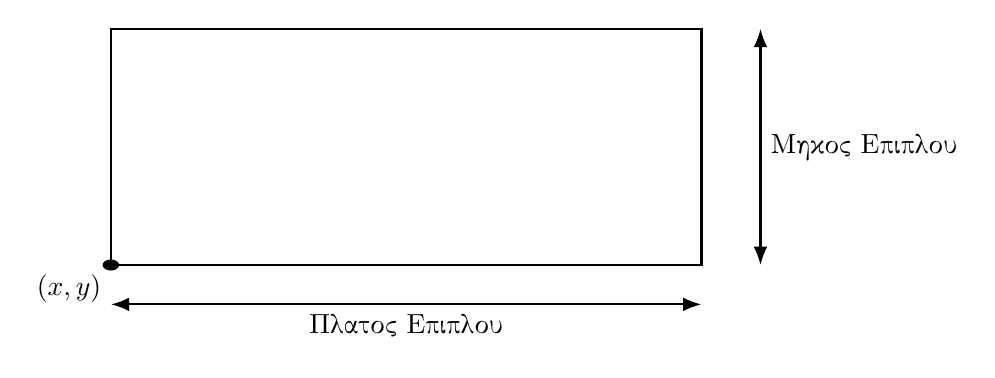
\begin{tikzpicture}[xscale = 1.5 , yscale = 1]
    \draw[thick] (0,0) rectangle (5,3);
    \draw[thick , Latex - Latex] (0, -0.5) -- (5, -0.5) node[midway , below]{Πλατος Επιπλου};
    \draw[thick , Latex - Latex] (5.5,0) -- (5.5, 3) node[midway ,right]{Μηκος Επιπλου};
    \fill[black] (0,0) circle (2pt); % Κουκκίδα
    \node[below left] at (0,0) {$(x, y)$}; % Ετικέτα
\end{tikzpicture}
\\
\newline
Αρα απο το (x,y) θα σχεδιασουμε ενα rectangle  με πλατος και μηκος οσο του αντιστοιχου επιπλου.\\
\newline
Οταν το $θ = \frac{π}{2}$ τοτε το αρχικο παραλληλογραμμο εχει περιστραφει κατα 90 μοιρες δεξιοστροφα και το σημειο (x,y) θα αντιστοιχει στο πανω αριστερο σημειο του rectangle.\\
\newline
\begin{tikzpicture}[xscale = 1 , yscale = 1.5]
    \draw[thick] (0,0) rectangle (5,3);
    \draw[thick , Latex - Latex] (0, -0.5) -- (5, -0.5) node[midway , below]{Μηκος Επιπλου};
    \draw[thick , Latex - Latex] (5.5,0) -- (5.5, 3) node[midway ,right]{Πλατος Επιπλου};
    \fill[black] (0,3) circle (2pt); % Κουκκίδα
    \node[above left] at (0,3) {$(x, y)$}; % Ετικέτα
\end{tikzpicture}\\
\newline
Αντιστοιχα οταν το $θ = π$ το (x,y) θα ειναι το πανω δεξιο σημειο του παραλληλογραμου και θα συμβολιζε οπως και πριν το σημειο εναρξης σχεδιασμου του επιπλου.\\
\newline
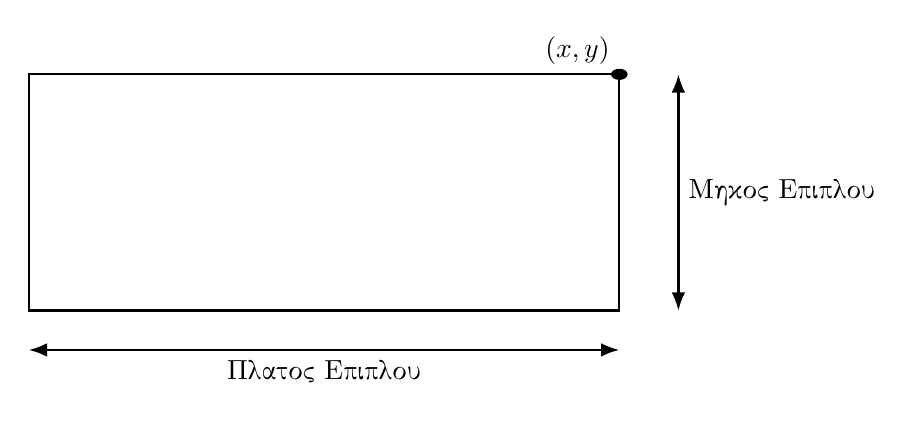
\begin{tikzpicture}[xscale = 1.5 , yscale = 1]
    \draw[thick] (0,0) rectangle (5,3);
    \draw[thick , Latex - Latex] (0, -0.5) -- (5, -0.5) node[midway , below]{Πλατος Επιπλου};
    \draw[thick , Latex - Latex] (5.5,0) -- (5.5, 3) node[midway ,right]{Μηκος Επιπλου};
    \fill[black] (5,3) circle (2pt); % Κουκκίδα
    \node[above left] at (5,3) {$(x, y)$}; % Ετικέτα
\end{tikzpicture}\\
\newline
Τελος οταν το $θ = \frac{3π}{2}$ τοτε το αρχικο παραλληλογραμμο εχει περιστραφει κατα $270$ μοιρες και το σημειο (x,y) θα αντιστοιχει στο κατω δεξιο σημειο του rectangle. \\
\newline
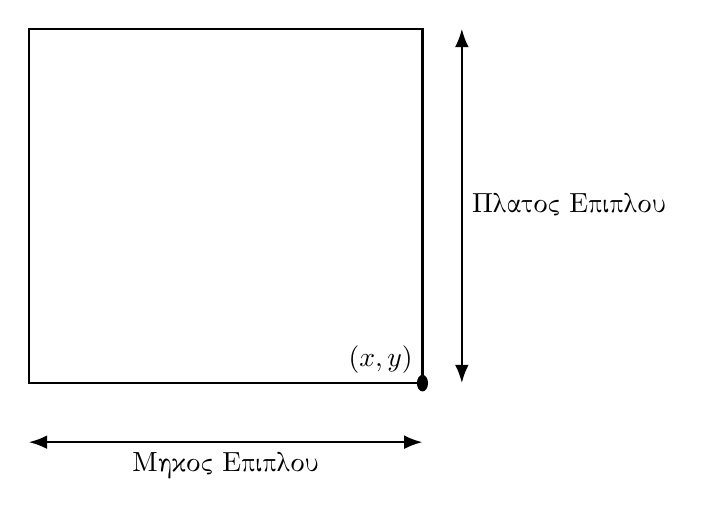
\begin{tikzpicture}[xscale = 1 , yscale = 1.5]
    \draw[thick] (0,0) rectangle (5,3);
    \draw[thick , Latex - Latex] (0, -0.5) -- (5, -0.5) node[midway , below]{Μηκος Επιπλου};
    \draw[thick , Latex - Latex] (5.5,0) -- (5.5, 3) node[midway ,right]{Πλατος Επιπλου};
    \fill[black] (5,0) circle (2pt); % Κουκκίδα
    \node[above left] at (5,0) {$(x, y)$}; % Ετικέτα
\end{tikzpicture}\\
\newline
Το δωματιο εχει τεσσερεις τοιχους , ο αριστερος βρισκεται στο $x = 0$ και $y \ne 0$ , ο δεξιος βρισκεται στο $x = 300$ και $y \ge 0$ , ο μπροστα(ετσι οπως μπαινουμε στο δωματιο) βρισκεται στο $x \ge 0 $ και $y = 400$ και τελος ο πισω τοιχος βρισκεται στο $x \ge 0$ και $y = 0$.\\
\newline
Παραδειγμα:\\
\newline
Ας πουμε οτι εξεταζουμε το κρεβατι σαν επιπλο που εχει Χ = 100 και Y = 200 και περνει σαν τιμη απο το domain του την (0 , 100 , 0). Τοτε επειδη το θ = 0 βρισκομαστε στην πρωτη περιπτωση και το παραλληλογραμμο θα ξεκιναει απο το (0 ,100). Αρα το rectangle που θα προκυψει και θα ικανοποιει τον περιορισμο οτι το κρεβατι θα ειναι κολιμενο σε εναν τουλαχιστον τοιχο(εδω στον αριστερο) θα ειναι:\\
\newline
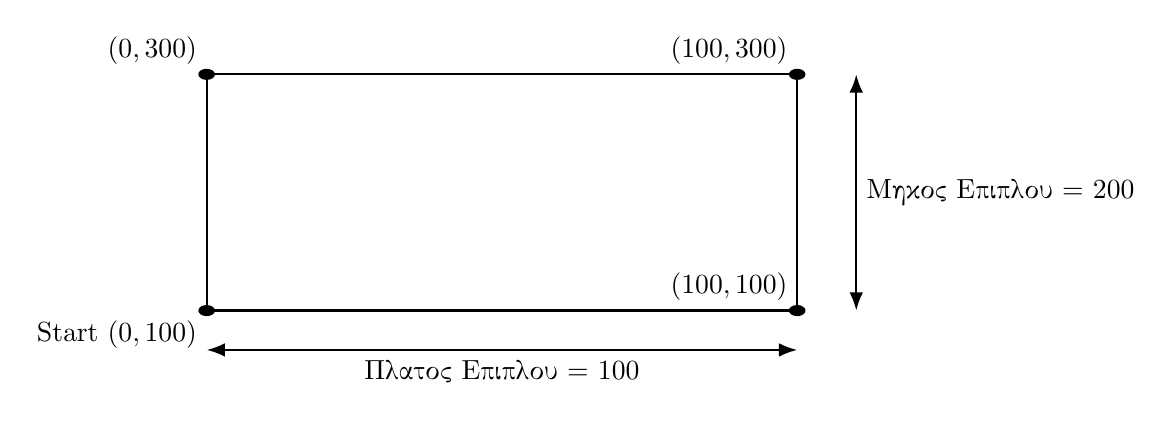
\begin{tikzpicture}[xscale = 1.5 , yscale = 1]
    \draw[thick] (0,0) rectangle (5,3);
    \draw[thick , Latex - Latex] (0, -0.5) -- (5, -0.5) node[midway , below]{Πλατος Επιπλου = 100};
    \draw[thick , Latex - Latex] (5.5,0) -- (5.5, 3) node[midway ,right]{Μηκος Επιπλου = 200};
    \fill[black] (5,3) circle (2pt); % Κουκκίδα
    \node[above left] at (5,3) {$(100, 300)$}; % Ετικέτα
    \fill[black] (0,0) circle (2pt); % Κουκκίδα
    \node[below left] at (0,0) { Start $(0, 100)$}; % Ετικέτα
   \fill[black] (0,3) circle (2pt); % Κουκκίδα
    \node[above left] at (0,3) {$(0, 300)$}; % Ετικέτα
    \fill[black] (5,0) circle (2pt); % Κουκκίδα
    \node[above left] at (5,0) {$(100 , 100)$}; % Ετικέτα
\end{tikzpicture}\\
\newline
Αρα αναλογα με την γωνια θ το επιπλο θα ξεκιναει απο διαφορετικο σημειο. Αρα οι περιορισμοι που θα παρω θα αφορουν ολες τις γωνιες θ.\\
\newline
\underline{Περιορισμοι}:\\
\newline
Πρεπει να ικανοποιησουμε $3$ περιορισμους:\\
$\bullet$ Το κρεβάτι θα πρέπει να είναι κολλημένο σε ένα από τους τοίχους.\\
$\bullet$ Το γραφείο θα πρέπει να είναι κολλημένο σε τοίχο και απέναντι από την είσοδο
φωτός στο δωμάτιο (μπαλκονόπορτα).\\
$\bullet$ Τα έπιπλα δεν πρέπει να εφάπτονται ή να πατάνε το ένα πάνω στο άλλο.\\
\newline
Επισης η πορτα θα πρεπει να ανοιγει.(Θεωρω οτι η πορτα ειναι ενα παραλληλογραμμο πλατους 100 και μηκους 100)\\
\newline
Οπως μπαινουμε μεσα στο δωματιο εχουμε:
\\
\newline
Αριστερος τοιχος: $x = 0 \wedge y \in [0,400]$\\Δεξιος τοιχος: $x = 300 \wedge y\in [0,400]$\\Μπροστα τοιχος: $x \in [0,300] \wedge y = 400$\\Πισω τοιχος: $x \in [0,300] \wedge y = 0$\\
\newline
\underline{Περιορισμος 1}:\\
\newline
Για να εφαπτεπται το κρεβατι με διαστασεις X = 100 και Y = 200 σε τουλαχιστον ενα τοιχο οταν μας δινεται μια τιμη της μεταβλτης $X_1$ της μορφης (x,y,θ) θα πρεπει να ισχυει(αναλογα με την τιμη της γωνιας θ) μια απο τις παρακατω συνθηκες:\\
\newline
Οι παρακατω περιορισμοι λαμβανουν υποψη και οτι το κρεβατι δεν πρεπει να εισαχθει σε σημειο που να μην ανοιγει η πορτα.\\
\newline
$\bullet$ Αν $θ = 0$ (δηλαδη το παραλληλογραμμο ξεκιναει απο το κατω αριστερο σημειο):\\
\newline
($x = 0$ και $100\le y \le200 $)(Αριστερο τοιχο) Ή ($x = 200$ και $0\le y \le200 $)(Δεξι τοιχο) Ή ($y = 200$ και $0\le x \le300 $)(Μπροστα τοιχο) Ή ($y = 0$ και $100\le x \le200 $)(Πισω τοιχο).\\
\newline
Για παραδειγμα την περιπτωση που $x = 0$ και $y = 100$ την εχουμε παρουσιασει πιο πανω και το παραλληλογραμμο εφαπτεται στον αριστερο τοιχο($x = 0$).\\
\newline
$\bullet$ Αν $θ = \frac{π}{2}$  (δηλαδη το παραλληλογραμμο ξεκιναει απο το πανω αριστερο σημειο και εχει περιστραφει κατα 90 μοιρες αρα το πλατος του κρεβατιου ειναι $200$ και το μηκος του $100$ ):\\
\newline
($x = 0$ και $200\le y \le400 $)(Αριστερο τοιχο) Ή ($x = 100$ και $100\le y \le400 $)(Δεξι τοιχο) Ή ($y = 400$ και $0\le x \le100 $)(Μπροστα τοιχο) Ή ($y = 100$ και $x = 100$)(Πισω τοιχο).\\
\newline
Για παραδειγμα οταν το $y = 100$ και $x = 100$ ικανοποιειται ο περιορισμος οτι το κρεβατι ακουμπαει σε τουλαχιστον ενα τοιχο διοτι ακουμπαει στον κατω. Ο λογος που το x και το y πρεπει να ειναι $100$ για να συμβαινει αυτο ειναι οτι εαν το x και το y  ηταν μικροτερα του $100$ τοτε δεν θα ανοιγε η πορτα , επισης το y δεν πρεπει να ειναι μεγαλυτερο του $100$ διοτι το πλατος του κρεβατιου ειναι $X = 100$ και επειδη το εχουμε περιστρεψει κατα $90$ μοιρες(δηλαδη το πλατος του κρεβατιου ειναι πλεον το $200$ και το μηκος του το $100$) θα πρεπει για να ακουμπαει στον Πισω τοιχο το y να ειναι $100$ , εαν $y >100$ τοτε $y -X > 100 -X  = 0 $ αρα δεν ακουμπαει στον Πισω τοιχο . Τελος το $x = 100$ γιατι εαν ειναι μεγαλυτερο το κρεβατι θα βγαινει εκτος των επιτρεπτων οριων του σπιτιου(Εχουμε μηκος κρεβατιου ισο με $200$ αρα εαν το $x > 100$ τοτε $x + Y > 100 + Y  = 300$). Αρα για ακουμπαει το κρεβατι στον Πισω τοιχο οταν ειναι γυρισμενο κατα $90$ μοιρες θα πρεπει το $x = 100$ και το  $y = 100$ . Με παρομοιο τροπο προκιπτουν οι σχεσεις και για τους υπολοιπους τρεις τοιχους.\\
\newline
$\bullet$ Αν $θ = π$  (δηλαδη το παραλληλογραμμο ξεκιναει απο το πανω δεξιο σημειο):\\
\newline
($x = 100$ και $300\le y \le400 $)(Αριστερο τοιχο) Ή ($x = 300$ και $200\le y \le400 $)(Δεξι τοιχο) Ή ($y = 400$ και $100\le x \le400 $)(Μπροστα τοιχο) Ή ($y = 200$ και $ 200 \le x \le 300$)(Πισω τοιχο).\\
\newline
$\bullet$ Αν $θ = \frac{3π}{2}$  (δηλαδη το παραλληλογραμμο ξεκιναει απο το κατω δεξιο σημειο):\\
\newline
($x = 200$ και $100\le y \le300 $)(Αριστερο τοιχο) Ή ($x = 300$ και $0\le y \le300 $)(Δεξι τοιχο) Ή ($y = 300$ και $ 200\le x\le 400 $)(Μπροστα τοιχο) Ή ($y = 0$ και $x = 300$)(Πισω τοιχο).\\
\newline
Αρα για την αντοιστοιχη τιμη του θ εαν ισχυει απο αυτες τις συνθηκες τοτε το κρεβατι εφαπτεται σε τουλαχιστον ενα τοιχο(πχ για $θ = \frac{3π}{2}$ και $y = 0$ και $x = 300$ τοτε το κρεβατι ακουμπαει και στον πισω τοιχο αλλα και στον δεξι).\\
\newline
\underline{Περιορισμος 2}:\\
\newline
Για να ειναι το γραφειο με διαστασεις $X = 160$ και $Y = 80$ κολλημενο σε τοιχο και απεναντι απο την μπαλκονοπορτα θα πρεπει ουσιαστικα να βρισκεται κολλημενο στον δεξι τοιχο . Αυτο γινεται εαν ισχυει καποια απο τις παρακατω συνθηκες για τις διαφορες τιμες του θ.\\
\newline
$\bullet$ Αν $θ = 0$ (δηλαδη το παραλληλογραμμο ξεκιναει απο το κατω αριστερο σημειο):\\
\newline
($x = 140$ και $0\le y \le320 $)\\
\newline
Οταν το θ ειναι $0$ για να ειναι το γραφειο κολλημενο στον δεξι τοιχο θα πρεπει το x να ειναι $140$ διοτι $140 + 160 = 300$ και το y θα πρεπει να παρει μια τιμη στο διαστημα [$0$ , $320$] προκειμενου να ισχυει οτι $y + 80 <=400$. Ομοιως και για τα υπολοιπα απλος οταν $θ =\frac{π}{2}$ ή $θ = \frac{3π}{2}$ τοτε το γραφειο εχει πλατος $80$ και μηκος $160$.\\
\newline
$\bullet$ Αν $θ = \frac{π}{2}$ (δηλαδη το παραλληλογραμμο ξεκιναει απο το πανω αριστερο σημειο):\\
\newline
($x = 220$ και $160\le y \le400 $)\\
\newline
$\bullet$ Αν $θ = π$ (δηλαδη το παραλληλογραμμο ξεκιναει απο το πανω δεξιο σημειο):\\
\newline
($x = 300$ και $80\le y \le400 $)\\
\newline
$\bullet$ Αν $θ = \frac{3π}{2}$ (δηλαδη το παραλληλογραμμο ξεκιναει απο το κατω δεξιο σημειο):\\
\newline
($x = 300$ και $0\le y \le 240 $)\\
\newline
\underline{Περιορισμος 3}:\\
\newline
Για να καταλαβουμε εαν δυο επιπλα εφαπτονται ή βρισκεται το ενα πανω στο αλλο θα πρεπει να βρουμε αρχικα τα ζευγαρια συντεταγμενων $(l_1.x$  , $l_1.y) $ και $(r_1.x$ , $r_2.y)$ οπου $l_1$ και $r_1$ ειναι το πανω αριστερο και το κατω δεξιο σημειο αντιστοιχα του πρωτου παραλληλογραμμου. Θα πρεπει να βρουμε και τα $l_2$ και $r_2$ σημεια του δευτερου παραλληλογραμμου.\\
\newline
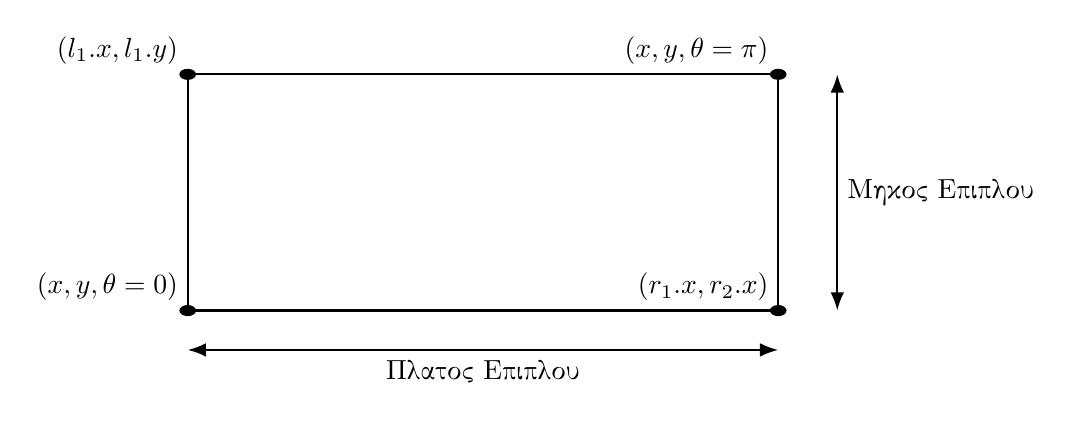
\begin{tikzpicture}[xscale = 1.5 , yscale = 1]
    \draw[thick] (0,0) rectangle (5,3);
    \draw[thick , Latex - Latex] (0, -0.5) -- (5, -0.5) node[midway , below]{Πλατος Επιπλου};
    \draw[thick , Latex - Latex] (5.5,0) -- (5.5, 3) node[midway ,right]{Μηκος Επιπλου};
    \fill[black] (0,0) circle (2pt); % Κουκκίδα
    \node[above left] at (0,0) {$(x , y ,θ=0 )$}; % Ετικέτα
    \fill[black] (5,3) circle (2pt); % Κουκκίδα
    \node[above left] at (5,3) {$(x , y ,θ=π )$}; % Ετικέτα
    \fill[black] (0,3) circle (2pt); % Κουκκίδα
    \node[above left] at (0,3) {$(l_1.x, l_1.y)$}; % Ετικέτα
    \fill[black] (5,0) circle (2pt); % Κουκκίδα
    \node[above left] at (5,0) {$(r_1.x , r_2.x)$}; % Ετικέτα
\end{tikzpicture}\\
\newline
\begin{tikzpicture}[xscale = 1 , yscale = 1.5]
    \draw[thick] (0,0) rectangle (5,3);
    \draw[thick , Latex - Latex] (0, -0.5) -- (5, -0.5) node[midway , below]{Μηκος Επιπλου};
    \draw[thick , Latex - Latex] (5.5,0) -- (5.5, 3) node[midway ,right]{Πλατος Επιπλου};
    \fill[black] (0,3) circle (2pt); % Κουκκίδα
    \node[above left] at (0,3) {$(x, y , θ = \frac{π}{2})$}; % Ετικέτα
    \fill[black] (5,0) circle (2pt); % Κουκκίδα
    \node[above left] at (5,0) {$(x, y , θ = \frac{3π}{2})$}; % Ετικέτα
\end{tikzpicture}\\
\newline
Αναλογα με την τιμη του θ βρισκουμε τα $l_1$ και $r_1$ και τα $l_2$ και $r_2$ ως εξης:\\
\newline
\underline{Πρωτο επιπλο με τιμη απο το domain (x,y,θ)}:\\
\newline
$\bullet$ Αν $θ = 0$ (δηλαδη το παραλληλογραμμο ξεκιναει απο το κατω αριστερο σημειο):\\
\newline
$l_1 = (x$ , $y +$ μηκος του επιπλου$)$\\
$r_1 = (x +$ πλατος του επιπλου , $y)$\\
\newline
$\bullet$ Αν $θ = \frac{π}{2}$ (δηλαδη το παραλληλογραμμο ξεκιναει απο το πανω αριστερο σημειο):\\
\newline
$l_1 = (x$ , $y)$\\
$r_1 = (x +$ μηκος του επιπλου , $y + $ πλατους του επιπλου$)$\\
\newline
$\bullet$ Αν $θ = π$ (δηλαδη το παραλληλογραμμο ξεκιναει απο το πανω δεξιο σημειο):\\
\newline
$l_1 = (x - $ πλατος του επιπλου , $y)$\\
$r_1 = (x $, $y - $ μηκος του επιπλου$)$\\
\newline
$\bullet$ Αν $θ = \frac{3π}{2}$ (δηλαδη το παραλληλογραμμο ξεκιναει απο το κατω δεξιο σημειο):\\
\newline
$l_1 = (x - $ μηκος του επιπλου , $y$ + πλατος του επιπλου$)$\\
$r_1 = (x $, $y)$\\
\newline
Ομοιως βρισκουμε και τα $l_2$ και $r_2$ για το δευτερο επιπλο.\\
\newline
Για να μην εφαπτονται και να μην βρισκεται το ενα επιπλο πανω στο αλλο θα πρεπει να ισχυει μια απο τις παρακατω δυο συνθηκες:\\
\newline
$\bullet$ $l_1.x > r_2.x$ Ή $l_2.x > r_1.x$\\
\newline
$\bullet$ $r_1.y > l_2.y$ Ή $r_2.y > l_1.y$\\
\newline
Αν δεν ισχυει καμια απο τις παραπανω σχεσεις τοτε τα επιπλα εφαπτονται ή βρισκονται το ενα πανω στο αλλο.\\
\newline
Τελος θα πρεπει να ελεγξουμε εαν καποιο απο τα επιπλα καρεκλα γραφειου ή καναπες εμποδιζει την πορτα του δωματιου(για τα αλλα δυο επιπλα ο ελεγχος αυτος γινεται μεσω των αντιστοιχων περιορισμων τους). Θεωρω οτι εαν ενα επιπλο τοποθετηθει στο $x=100$ η στο $y = 100$ τοτε ανοιγει η πορτα.\\
\newline
Οποτε θεωρωντας την πορτα σαν ενα παραλληλογραμμο πλατους $100$ και μηκους $100$ (δηλαδη $l_2.x = 0 , l_2.y = 100 , r_2.x = 100 , r_2.y = 0$)  και ενα επιπλο για το οποιο εχουμε υπολογισει τα ζευγαρια συντεταγμενων $l_1$ και $r_1$  , θα πρεπει για να μην εμποδιζουμε το ανοιγμα της πορτας να ισχυει μια απο τις παρακατω δυο συνθηκες:\\
\newline
$\bullet$ $l_1.x \ge 100$ Ή $0 \ge r_1.x$\\
\newline
$\bullet$ $r_1.y \ge 100$ Ή $ 0 \ge l_1.y$\\
\newline
Αυτοι ειναι ολοι οι περιορισμοι του προβληματος!!\\
\newline
Το συγκεκριμενο προβλημα ικανοποιησης περιορισμων εχει λυση. Mια αναθεση τιμων στις τεσσερις μεταβλητες που θα ικανοποιουσε ολους τους παραπανω περιορισμους ειναι η ακολουθη:\\
\newline
Κρεβατι: $(x = 150$ , $ y =0$ , $θ = 0)$ (Ειναι κολλημενο στον πισω τοιχο)\\
Γραφειο: $(x = 140$ , $ y =320$ , $θ = 0)$ (Βρισκεται απεναντι απο την μπαλκονοπορτα και μια πλευρα του ειναι κολλημενη σε τοιχο και συγκεκριμενα στον δεξι)\\
Καναπες: $(x = 0$ , $ y =400$ , $θ = \frac{π}{2})$ (Δεν εφαπτεται με καποιο αλλο επιπλο)\\
Καρεκλα: $(x = 150$ , $ y =250$ , $θ = 0)$ (Δεν εφαπτεται με καποιο αλλο επιπλο)\\
\newline
Κανενα επιπλο δεν εφαπτεται ή βρισκεται πανω απο καποιο αλλο  , η πορτα ανοιγει κανονικα και πληρουνται ολοι οι περιορισμοι.\\
\newline
\newpage
\textbf{\Large\textit{\underline{Πρόβλημα $3$}}:}\\
\newline
$\bullet$ Μοντελοποιηση Προβληματος:\\
\newline
Εχουμε $5$ μεταβλητες τις $Α_1$ , $Α_2$ , $Α_3$ , $Α_4$ , $Α_5$ μια για καθε ενεργεια.\\
\newline
Το domain καθε μεταβλητες $A_i$ ειναι: $A_i = \{ $9:00 , 10:00 , 11:00$\}$\\
\newline
Περιορισμοι προβληματος:\\
\newline
$\bullet$ Η $Α_1$ πρεπει να αρχισει μετα την $A_3$ $\Longrightarrow $ $A_1 > A_3$\\
$\bullet$ Η $Α_3$ πρέπει να αρχίσει πριν την $A_4$ και μετά την $Α_5$ $\Longrightarrow $ $A_5 < A_3 < A_4$\\
$\bullet$ Η $Α_2$ δεν μπορεί να εκτελείται την ίδια ώρα με την $Α_1$ ή την $Α_4$ $\Longrightarrow $ $A_2 \ne A_1$ και $A_2 \ne A_4$\\
$\bullet$ Η $Α_4$ δεν μπορεί να αρχίσει στις 10:00 $\Longrightarrow $ $A_4 \ne $ 10:00\\
\newline
Neighbours καθε μεταβλητης:\\
\newline
$Α_1$: $A_3$ , $A_2$\\
$A_2$: $A_1$ , $A_4$\\
$A_3$: $A_1$ , $A_4$ , $A_5$\\
$A_4$: $A_2$ , $A_3$\\
$A_5$: $A_3$\\
\newline
Εαν μια μεταβλητη $A_i$ εχει περιορισμο με μια μεταβλητη $A_j$ τοτε και η $A_i$ ειναι γειτονας με την $A_j$ αλλα και η $A_j$ ειναι γειτονας με την $A_i$.\\
\newline
\newpage
\begin{itemize}
\item Γραφος Περιορισμων:\\
\begin{center}
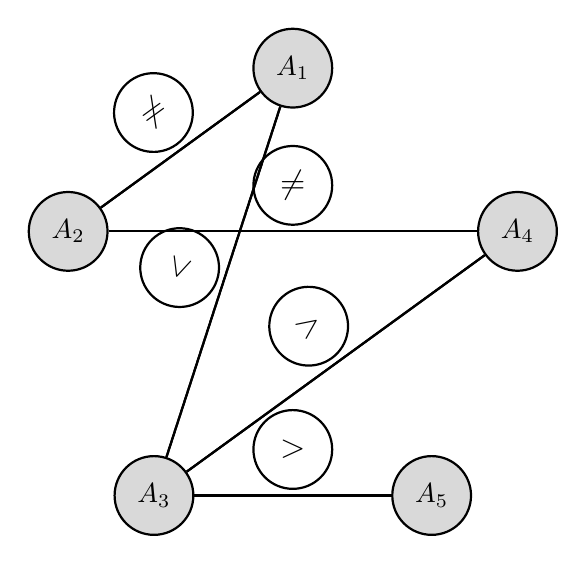
\begin{tikzpicture}[node distance=2cm, every node/.style={circle, draw, minimum size=1cm, inner sep=0pt}, thick]

% Nodes placed in a pentagon shape
\node[fill=gray!30] (A1) at (90:3cm) {$A_1$}; % Top
\node[fill=gray!30] (A2) at (162:3cm) {$A_2$}; % Top-left
\node[fill=gray!30] (A3) at (234:3cm) {$A_3$}; % Bottom-left
\node[fill=gray!30] (A5) at (306:3cm) {$A_5$}; % Bottom-right
\node[fill=gray!30] (A4) at (18:3cm) {$A_4$}; % Top-right

% Edges following the graph structure
\draw (A1) -- (A2);
\draw (A1) -- (A3);
\draw (A2) -- (A4);
\draw (A3) -- (A4);
\draw (A3) -- (A5);
\draw (A1) -- (A2) node[sloped,midway,above=0.2em] {\large $\ne$};
\draw (A2) -- (A4) node[sloped,midway,above=0.2em] {\large $\ne$};
\draw (A1) -- (A3) node[sloped,midway,above=0.2em] {\large $<$};
\draw (A4) -- (A3) node[sloped,midway,above=0.2em] {\large $>$};
\draw (A3) -- (A5) node[sloped,midway,above=0.2em] {\large $>$};
\end{tikzpicture}
\end{center}
\end{itemize}
Στον γραφο περιορισμων εισαγουμε μια ακμη $A_i - A_j$ εαν το $A_i$ ειναι γειτονας με το $A_j$ δηλαδη συνδεονται σε καποιο περιορισμο. Ο γραφος ειναι μη κατευθυνομενος δηλαδη μπορουμε να παμε και απο το $A_i$ στο $A_j$ αλλα και απο το $A_j$ στο $A_i$. Για καθε ακμη εχω προσθεσει σαν βαρος τον περιορισμο που τις συνδεει. Για παραδειγμα στην ακμη $A_1 - A_2$ εχουμε το συμβολο $\ne$ γιατι με βαση τον τριτο περιορισμο θα πρεπει το $A_1 \ne A_2$ , το ιδιο ισχυει και για την ακμη $A_2 - A_1$ , δηλαδη $A_2 \ne A_1$ .\\
\newline
$\bullet$ AC-3\\
\newline
Αρχικα τα domains των μεταβλητων ειναι γεματα\\
\newline
$A_1 = \{ $9:00 , 10:00 , 11:00$\}$\\
$A_2 = \{ $9:00 , 10:00 , 11:00$\}$\\
$A_3 = \{ $9:00 , 10:00 , 11:00$\}$\\
$A_4 = \{ $9:00 , 10:00 , 11:00$\}$\\
$A_5 = \{ $9:00 , 10:00 , 11:00$\}$\\
\newline
Εχουμε μια ουρα στην οποια εισαγουμε στην αρχη  καθε ακμη του γραφου περιορισμου. Καθε φορα που θα βγαζουμε μια ακμη $A_i - A_j$ απο την ουρα θα ξαναεισαγουμε ολες τις ακμες της μορφης $A_k-A_i$ οι οποιες δεν ειναι ειδη μεσα στο queue.\\
\newline
$\bullet$ [ $(A_1 , A_3)$ , $(A_3 , A_1)$ , $(A_3 , A_4)$ , $(A_4 , A_3)$ , $(A_3 , A_5)$ , $(A_5 , A_3)$ , $(A_2 , A_1)$ , $(A_1 , A_2)$ , $(A_2 , A_4)$  , $(A_4 , A_2)$ ]\\
\newline
$\bullet$ Βγαζουμε την ακμη $(A_1 , A_3)$  και ελεγχουμε $\forall x \in domain A_1$ , αν $\exists$  $y \in domain A_3$ ετσι ωστε να ικανοποιουνται ολοι οι περιορισμοι μεταξυ των $A_1$ και $A_3$ . Αν για μια τιμη x δεν υπαρχει τιμη y τοτε διαγραφουμε το x απο το πεδιο τιμων της $A_1$ . Επειδη για την τιμη $9$ στο πεδιο της $A_1$ δεν υπαρχει τιμη στο πεδιο της $A_3$ για την οποια να ισχυει $9 > y$ διαγραφουμε το $9$ απο το domain της $A_1$ . Δεν ξαναεισαγουμε καποια αλλη ακμη στην ουρα γιατι υπαρχει ειδη μεσα η $(A_3 , A_1)$  και η $(A_2 , A_1)$. Τα ανανεωμενα domains των μεταβλητων και η καινουργια ουρα ειναι η παρακατω: \\
\newline
$A_1 = \{ $\cancel{9:00} , 10:00 , 11:00$\}$\\
$A_2 = \{ $9:00 , 10:00 , 11:00$\}$\\
$A_3 = \{ $9:00 , 10:00 , 11:00$\}$\\
$A_4 = \{ $9:00 , 10:00 , 11:00$\}$\\
$A_5 = \{ $9:00 , 10:00 , 11:00$\}$\\
\newline
[ \cancel{$(A_1 , A_3)$} , $(A_3 , A_1)$ , $(A_3 , A_4)$ , $(A_4 , A_3)$ , $(A_3 , A_5)$ , $(A_5 , A_3)$ , $(A_2 , A_1)$ , $(A_1 , A_2)$ , $(A_2 , A_4)$  , $(A_4 , A_2)$ ]\\
\newline
$\bullet$ Βγαζουμε την ακμη  $(A_3 , A_1)$ και φευγει το $11$ απο το πεδιο τιμων της $A_3$ αφου δεν υπαρχει τιμη στο πεδιο τιμων της $A_1$ που να ικανοποιει τον περιορισμο μεταξυ της $A_3$ και $A_1$ ($Α_3 < Α_1$). Ξαναεισαγουμε την ακμη  $(A_1 , A_3)$\\
\newline
$A_1 = \{ $\cancel{9:00} , 10:00 , 11:00$\}$\\
$A_2 = \{ $9:00 , 10:00 , 11:00$\}$\\
$A_3 = \{ $9:00 , 10:00 , \cancel{11:00}$\}$\\
$A_4 = \{ $9:00 , 10:00 , 11:00$\}$\\
$A_5 = \{ $9:00 , 10:00 , 11:00$\}$\\
\newline
[ \cancel{$(A_1 , A_3)$} , \cancel{$(A_3 , A_1)$} , $(A_3 , A_4)$ , $(A_4 , A_3)$ , $(A_3 , A_5)$ , $(A_5 , A_3)$ , $(A_2 , A_1)$ , $(A_1 , A_2)$ , $(A_2 , A_4)$  , $(A_4 , A_2)$ , $(A_1 , A_3)$ ]\\
\newline
$\bullet$ Βγαζουμε την ακμη  $(A_3 , A_4)$ δεν φευγει καποια τιμη απο το πεδιο τιμων της $A_3$.\\
\newline
$A_1 = \{ $\cancel{9:00} , 10:00 , 11:00$\}$\\
$A_2 = \{ $9:00 , 10:00 , 11:00$\}$\\
$A_3 = \{ $9:00 , 10:00 , \cancel{11:00}$\}$\\
$A_4 = \{ $9:00 , 10:00 , 11:00$\}$\\
$A_5 = \{ $9:00 , 10:00 , 11:00$\}$\\
\newline
[ \cancel{$(A_1 , A_3)$} , \cancel{$(A_3 , A_1)$} , \cancel{$(A_3 , A_4)$} , $(A_4 , A_3)$ , $(A_3 , A_5)$ , $(A_5 , A_3)$ , $(A_2 , A_1)$ , $(A_1 , A_2)$ , $(A_2 , A_4)$  , $(A_4 , A_2)$ , $(A_1 , A_3)$ ]\\
\newline
$\bullet$ Βγαζουμε την ακμη  $(A_4 , A_3)$ και φευγει το $9$ απο το πεδιο τιμων της $A_4$ αφου δεν υπαρχει τιμη στο πεδιο τιμων της $A_3$ που να ικανοποιει τον περιορισμο μεταξυ της $A_4$ και $A_3$ ($Α_4 > Α_3$). Ξαναεισαγουμε την ακμη  $(A_3 , A_4)$\\
\newline
$A_1 = \{ $\cancel{9:00} , 10:00 , 11:00$\}$\\
$A_2 = \{ $9:00 , 10:00 , 11:00$\}$\\
$A_3 = \{ $9:00 , 10:00 , \cancel{11:00}$\}$\\
$A_4 = \{ $ \cancel{9:00} , 10:00 , 11:00$\}$\\
$A_5 = \{ $9:00 , 10:00 , 11:00$\}$\\
\newline
[ \cancel{$(A_1 , A_3)$} , \cancel{$(A_3 , A_1)$} , \cancel{$(A_3 , A_4)$} , \cancel{$(A_4 , A_3)$} , $(A_3 , A_5)$ , $(A_5 , A_3)$ , $(A_2 , A_1)$ , $(A_1 , A_2)$ , $(A_2 , A_4)$  , $(A_4 , A_2)$ , $(A_1 , A_3)$ , $(A_3 , A_4)$  ]\\
\newline
$\bullet$ Βγαζουμε την ακμη  $(A_3 , A_5)$ και φευγει το $9$ απο το πεδιο τιμων της $A_3$ αφου δεν υπαρχει τιμη στο πεδιο τιμων της $A_5$ που να ικανοποιει τον περιορισμο μεταξυ της $A_3$ και $A_5$ ($Α_3 > Α_5$). Ξαναεισαγουμε την ακμη  $(A_4 , A_3)$\\
\newline
$A_1 = \{ $\cancel{9:00} , 10:00 , 11:00$\}$\\
$A_2 = \{ $9:00 , 10:00 , 11:00$\}$\\
$A_3 = \{ $ \cancel{9:00} , 10:00 , \cancel{11:00}$\}$\\
$A_4 = \{ $ \cancel{9:00} , 10:00 , 11:00$\}$\\
$A_5 = \{ $9:00 , 10:00 , 11:00$\}$\\
\newline
[ \cancel{$(A_1 , A_3)$} , \cancel{$(A_3 , A_1)$} , \cancel{$(A_3 , A_4)$} , \cancel{$(A_4 , A_3)$} , \cancel{$(A_3 , A_5)$} , $(A_5 , A_3)$ , $(A_2 , A_1)$ , $(A_1 , A_2)$ , $(A_2 , A_4)$  , $(A_4 , A_2)$ , $(A_1 , A_3)$ , $(A_3 , A_4)$ , $(A_4 , A_3)$ ]\\
\newline
$\bullet$ Βγαζουμε την ακμη  $(A_5 , A_3)$ και φευγει το $10$ και το $11$ απο το πεδιο τιμων της $A_5$ αφου δεν υπαρχει τιμη στο πεδιο τιμων της $A_3$ που να ικανοποιει τον περιορισμο μεταξυ της $A_5$ και $A_3$ ($Α_5 < Α_3$). Ξαναεισαγουμε την ακμη  $(A_3 , A_5)$\\
\newline
$A_1 = \{ $\cancel{9:00} , 10:00 , 11:00$\}$\\
$A_2 = \{ $9:00 , 10:00 , 11:00$\}$\\
$A_3 = \{ $ \cancel{9:00} , 10:00 , \cancel{11:00}$\}$\\
$A_4 = \{ $ \cancel{9:00} , 10:00 , 11:00$\}$\\
$A_5 = \{ $9:00 , \cancel{10:00} , \cancel{11:00} $\}$\\
\newline
[ \cancel{$(A_1 , A_3)$} , \cancel{$(A_3 , A_1)$} , \cancel{$(A_3 , A_4)$} , \cancel{$(A_4 , A_3)$} , \cancel{$(A_3 , A_5)$} , \cancel{$(A_5 , A_3)$} , $(A_2 , A_1)$ , $(A_1 , A_2)$ , $(A_2 , A_4)$  , $(A_4 , A_2)$ , $(A_1 , A_3)$ , $(A_3 , A_4)$ , $(A_4 , A_3)$ , $(A_3 , A_5)$ ]\\
\newline
$\bullet$ Βγαζουμε την ακμη  $(A_2 , A_1)$ δεν φευγει καποια τιμη απο το πεδιο τιμων της $A_2$.\\
\newline
$A_1 = \{ $\cancel{9:00} , 10:00 , 11:00$\}$\\
$A_2 = \{ $9:00 , 10:00 , 11:00$\}$\\
$A_3 = \{ $ \cancel{9:00} , 10:00 , \cancel{11:00}$\}$\\
$A_4 = \{ $ \cancel{9:00} , 10:00 , 11:00$\}$\\
$A_5 = \{ $9:00 , \cancel{10:00} , \cancel{11:00} $\}$\\
\newline
[ \cancel{$(A_1 , A_3)$} , \cancel{$(A_3 , A_1)$} , \cancel{$(A_3 , A_4)$} , \cancel{$(A_4 , A_3)$} , \cancel{$(A_3 , A_5)$} , \cancel{$(A_5 , A_3)$} , \cancel{$(A_2 , A_1)$} , $(A_1 , A_2)$ , $(A_2 , A_4)$  , $(A_4 , A_2)$ , $(A_1 , A_3)$ , $(A_3 , A_4)$ , $(A_4 , A_3)$ , $(A_3 , A_5)$ ]\\
\newline
$\bullet$ Βγαζουμε την ακμη  $(A_1 , A_2)$ δεν φευγει καποια τιμη απο το πεδιο τιμων της $A_1$.\\
\newline
$A_1 = \{ $\cancel{9:00} , 10:00 , 11:00$\}$\\
$A_2 = \{ $9:00 , 10:00 , 11:00$\}$\\
$A_3 = \{ $ \cancel{9:00} , 10:00 , \cancel{11:00}$\}$\\
$A_4 = \{ $ \cancel{9:00} , 10:00 , 11:00$\}$\\
$A_5 = \{ $9:00 , \cancel{10:00} , \cancel{11:00} $\}$\\
\newline
[ \cancel{$(A_1 , A_3)$} , \cancel{$(A_3 , A_1)$} , \cancel{$(A_3 , A_4)$} , \cancel{$(A_4 , A_3)$} , \cancel{$(A_3 , A_5)$} , \cancel{$(A_5 , A_3)$} , \cancel{$(A_2 , A_1)$} , \cancel{$(A_1 , A_2)$} , $(A_2 , A_4)$  , $(A_4 , A_2)$ , $(A_1 , A_3)$ , $(A_3 , A_4)$ , $(A_4 , A_3)$ , $(A_3 , A_5)$ ]\\
\newline
$\bullet$ Βγαζουμε την ακμη  $(A_2 , A_4)$ δεν φευγει καποια τιμη απο το πεδιο τιμων της $A_2$.\\
\newline
$A_1 = \{ $\cancel{9:00} , 10:00 , 11:00$\}$\\
$A_2 = \{ $9:00 , 10:00 , 11:00$\}$\\
$A_3 = \{ $ \cancel{9:00} , 10:00 , \cancel{11:00}$\}$\\
$A_4 = \{ $ \cancel{9:00} , 10:00 , 11:00$\}$\\
$A_5 = \{ $9:00 , \cancel{10:00} , \cancel{11:00} $\}$\\
\newline
[ \cancel{$(A_1 , A_3)$} , \cancel{$(A_3 , A_1)$} , \cancel{$(A_3 , A_4)$} , \cancel{$(A_4 , A_3)$} , \cancel{$(A_3 , A_5)$} , \cancel{$(A_5 , A_3)$} , \cancel{$(A_2 , A_1)$} , \cancel{$(A_1 , A_2)$} , \cancel{$(A_2 , A_4)$}  , $(A_4 , A_2)$ , $(A_1 , A_3)$ , $(A_3 , A_4)$ , $(A_4 , A_3)$ , $(A_3 , A_5)$ ]\\
\newline
$\bullet$ Βγαζουμε την ακμη  $(A_4 , A_2)$ δεν φευγει καποια τιμη απο το πεδιο τιμων της $A_4$.\\
\newline
$A_1 = \{ $\cancel{9:00} , 10:00 , 11:00$\}$\\
$A_2 = \{ $9:00 , 10:00 , 11:00$\}$\\
$A_3 = \{ $ \cancel{9:00} , 10:00 , \cancel{11:00}$\}$\\
$A_4 = \{ $ \cancel{9:00} , 10:00 , 11:00$\}$\\
$A_5 = \{ $9:00 , \cancel{10:00} , \cancel{11:00} $\}$\\
\newline
[ \cancel{$(A_1 , A_3)$} , \cancel{$(A_3 , A_1)$} , \cancel{$(A_3 , A_4)$} , \cancel{$(A_4 , A_3)$} , \cancel{$(A_3 , A_5)$} , \cancel{$(A_5 , A_3)$} , \cancel{$(A_2 , A_1)$} , \cancel{$(A_1 , A_2)$} , \cancel{$(A_2 , A_4)$}  , \cancel{$(A_4 , A_2)$} , $(A_1 , A_3)$ , $(A_3 , A_4)$ , $(A_4 , A_3)$ , $(A_3 , A_5)$ ]\\
\newline
$\bullet$ Βγαζουμε την ακμη  $(A_1 , A_3)$ και φευγει το $10$ απο το πεδιο τιμων της $A_1$ αφου δεν υπαρχει τιμη στο πεδιο τιμων της $A_3$ που να ικανοποιει τον περιορισμο μεταξυ της $A_1$ και $A_3$ ($Α_1 > Α_3$). Ξαναεισαγουμε τις ακμες  $(A_3 , A_1)$ και $(A_2 , A_1)$ \\
\newline
$A_1 = \{ $\cancel{9:00} , \cancel{10:00} , 11:00$\}$\\
$A_2 = \{ $9:00 , 10:00 , 11:00$\}$\\
$A_3 = \{ $ \cancel{9:00} , 10:00 , \cancel{11:00}$\}$\\
$A_4 = \{ $ \cancel{9:00} , 10:00 , 11:00$\}$\\
$A_5 = \{ $9:00 , \cancel{10:00} , \cancel{11:00} $\}$\\
\newline
[ \cancel{$(A_1 , A_3)$} , \cancel{$(A_3 , A_1)$} , \cancel{$(A_3 , A_4)$} , \cancel{$(A_4 , A_3)$} , \cancel{$(A_3 , A_5)$} , \cancel{$(A_5 , A_3)$} , \cancel{$(A_2 , A_1)$} , \cancel{$(A_1 , A_2)$} , \cancel{$(A_2 , A_4)$}  , \cancel{$(A_4 , A_2)$} , \cancel{$(A_1 , A_3)$} , $(A_3 , A_4)$ , $(A_4 , A_3)$ , $(A_3 , A_5)$ , $(A_3 , A_1)$ , $(A_2 , A_1)$  ]\\
\newline
$\bullet$ Βγαζουμε την ακμη  $(A_3 , A_4)$ δεν φευγει καποια τιμη απο το πεδιο τιμων της $A_3$.  \\
\newline
$A_1 = \{ $\cancel{9:00} , \cancel{10:00} , 11:00$\}$\\
$A_2 = \{ $9:00 , 10:00 , 11:00$\}$\\
$A_3 = \{ $ \cancel{9:00} , 10:00 , \cancel{11:00}$\}$\\
$A_4 = \{ $ \cancel{9:00} , 10:00 , 11:00$\}$\\
$A_5 = \{ $9:00 , \cancel{10:00} , \cancel{11:00} $\}$\\
\newline
[ \cancel{$(A_1 , A_3)$} , \cancel{$(A_3 , A_1)$} , \cancel{$(A_3 , A_4)$} , \cancel{$(A_4 , A_3)$} , \cancel{$(A_3 , A_5)$} , \cancel{$(A_5 , A_3)$} , \cancel{$(A_2 , A_1)$} , \cancel{$(A_1 , A_2)$} , \cancel{$(A_2 , A_4)$}  , \cancel{$(A_4 , A_2)$} , \cancel{$(A_1 , A_3)$} , \cancel{$(A_3 , A_4)$} , $(A_4 , A_3)$ , $(A_3 , A_5)$ , $(A_3 , A_1)$ , $(A_2 , A_1)$  ]\\
\newline
$\bullet$ Βγαζουμε την ακμη  $(A_4 , A_3)$ και φευγει το $10$ απο το πεδιο τιμων της $A_4$ αφου δεν υπαρχει τιμη στο πεδιο τιμων της $A_3$ που να ικανοποιει τον περιορισμο μεταξυ της $A_4$ και $A_3$ ($Α_4 > Α_3$). Ξαναεισαγουμε τις ακμες  $(A_3 , A_4)$ και $(A_2 , A_4)$ \\
\newline
$A_1 = \{ $\cancel{9:00} , \cancel{10:00} , 11:00$\}$\\
$A_2 = \{ $9:00 , 10:00 , 11:00$\}$\\
$A_3 = \{ $ \cancel{9:00} , 10:00 , \cancel{11:00}$\}$\\
$A_4 = \{ $ \cancel{9:00} , \cancel{10:00} , 11:00$\}$\\
$A_5 = \{ $9:00 , \cancel{10:00} , \cancel{11:00} $\}$\\
\newline
[ \cancel{$(A_1 , A_3)$} , \cancel{$(A_3 , A_1)$} , \cancel{$(A_3 , A_4)$} , \cancel{$(A_4 , A_3)$} , \cancel{$(A_3 , A_5)$} , \cancel{$(A_5 , A_3)$} , \cancel{$(A_2 , A_1)$} , \cancel{$(A_1 , A_2)$} , \cancel{$(A_2 , A_4)$}  , \cancel{$(A_4 , A_2)$} , \cancel{$(A_1 , A_3)$} , \cancel{$(A_3 , A_4)$} , \cancel{$(A_4 , A_3)$} , $(A_3 , A_5)$ , $(A_3 , A_1)$ , $(A_2 , A_1)$ , $(A_3 , A_4)$ , $(A_2 , A_4)$ ]\\
\newline
$\bullet$ Βγαζουμε την ακμη  $(A_3 , A_5)$ δεν φευγει καποια τιμη απο το πεδιο τιμων της $A_3$.\\
\newline
$A_1 = \{ $\cancel{9:00} , \cancel{10:00} , 11:00$\}$\\
$A_2 = \{ $9:00 , 10:00 , 11:00$\}$\\
$A_3 = \{ $ \cancel{9:00} , 10:00 , \cancel{11:00}$\}$\\
$A_4 = \{ $ \cancel{9:00} , \cancel{10:00} , 11:00$\}$\\
$A_5 = \{ $9:00 , \cancel{10:00} , \cancel{11:00} $\}$\\
\newline
[ \cancel{$(A_1 , A_3)$} , \cancel{$(A_3 , A_1)$} , \cancel{$(A_3 , A_4)$} , \cancel{$(A_4 , A_3)$} , \cancel{$(A_3 , A_5)$} , \cancel{$(A_5 , A_3)$} , \cancel{$(A_2 , A_1)$} , \cancel{$(A_1 , A_2)$} , \cancel{$(A_2 , A_4)$}  , \cancel{$(A_4 , A_2)$} , \cancel{$(A_1 , A_3)$} , \cancel{$(A_3 , A_4)$} , \cancel{$(A_4 , A_3)$} , \cancel{$(A_3 , A_5)$} , $(A_3 , A_1)$ , $(A_2 , A_1)$ , $(A_3 , A_4)$ , $(A_2 , A_4)$ ]\\
\newline
$\bullet$ Βγαζουμε την ακμη  $(A_3 , A_1)$ δεν φευγει καποια τιμη απο το πεδιο τιμων της $A_3$.\\
\newline
$A_1 = \{ $\cancel{9:00} , \cancel{10:00} , 11:00$\}$\\
$A_2 = \{ $9:00 , 10:00 , 11:00$\}$\\
$A_3 = \{ $ \cancel{9:00} , 10:00 , \cancel{11:00}$\}$\\
$A_4 = \{ $ \cancel{9:00} , \cancel{10:00} , 11:00$\}$\\
$A_5 = \{ $9:00 , \cancel{10:00} , \cancel{11:00} $\}$\\
\newline
[ \cancel{$(A_1 , A_3)$} , \cancel{$(A_3 , A_1)$} , \cancel{$(A_3 , A_4)$} , \cancel{$(A_4 , A_3)$} , \cancel{$(A_3 , A_5)$} , \cancel{$(A_5 , A_3)$} , \cancel{$(A_2 , A_1)$} , \cancel{$(A_1 , A_2)$} , \cancel{$(A_2 , A_4)$}  , \cancel{$(A_4 , A_2)$} , \cancel{$(A_1 , A_3)$} , \cancel{$(A_3 , A_4)$} , \cancel{$(A_4 , A_3)$} , \cancel{$(A_3 , A_5)$} , \cancel{$(A_3 , A_1)$} , $(A_2 , A_1)$ , $(A_3 , A_4)$ , $(A_2 , A_4)$ ]\\
\newline
$\bullet$ Βγαζουμε την ακμη  $(A_2 , A_1)$ και φευγει το $11$ απο το πεδιο τιμων της $A_2$ αφου δεν υπαρχει τιμη στο πεδιο τιμων της $A_1$ που να ικανοποιει τον περιορισμο μεταξυ της $A_2$ και $A_1$ ($Α_2 \ne Α_1$). Ξαναεισαγουμε τις ακμες  $(A_1 , A_2)$ και $(A_4 , A_2)$ \\
\newline
$A_1 = \{ $\cancel{9:00} , \cancel{10:00} , 11:00$\}$\\
$A_2 = \{ $9:00 , 10:00 , \cancel{11:00}$\}$\\
$A_3 = \{ $ \cancel{9:00} , 10:00 , \cancel{11:00}$\}$\\
$A_4 = \{ $ \cancel{9:00} , \cancel{10:00} , 11:00$\}$\\
$A_5 = \{ $9:00 , \cancel{10:00} , \cancel{11:00} $\}$\\
\newline
[ \cancel{$(A_1 , A_3)$} , \cancel{$(A_3 , A_1)$} , \cancel{$(A_3 , A_4)$} , \cancel{$(A_4 , A_3)$} , \cancel{$(A_3 , A_5)$} , \cancel{$(A_5 , A_3)$} , \cancel{$(A_2 , A_1)$} , \cancel{$(A_1 , A_2)$} , \cancel{$(A_2 , A_4)$}  , \cancel{$(A_4 , A_2)$} , \cancel{$(A_1 , A_3)$} , \cancel{$(A_3 , A_4)$} , \cancel{$(A_4 , A_3)$} , \cancel{$(A_3 , A_5)$} , \cancel{$(A_3 , A_1)$} , \cancel{$(A_2 , A_1)$} , $(A_3 , A_4)$ , $(A_2 , A_4)$ , $(A_1 , A_2)$ , $(A_4 , A_2)$  ]\\
\newline
$\bullet$ Βγαζουμε την ακμη  $(A_3 , A_4)$ δεν φευγει καποια τιμη απο το πεδιο τιμων της $A_3$.\\
\newline
$A_1 = \{ $\cancel{9:00} , \cancel{10:00} , 11:00$\}$\\
$A_2 = \{ $9:00 , 10:00 , \cancel{11:00}$\}$\\
$A_3 = \{ $ \cancel{9:00} , 10:00 , \cancel{11:00}$\}$\\
$A_4 = \{ $ \cancel{9:00} , \cancel{10:00} , 11:00$\}$\\
$A_5 = \{ $9:00 , \cancel{10:00} , \cancel{11:00} $\}$\\
\newline
[ \cancel{$(A_1 , A_3)$} , \cancel{$(A_3 , A_1)$} , \cancel{$(A_3 , A_4)$} , \cancel{$(A_4 , A_3)$} , \cancel{$(A_3 , A_5)$} , \cancel{$(A_5 , A_3)$} , \cancel{$(A_2 , A_1)$} , \cancel{$(A_1 , A_2)$} , \cancel{$(A_2 , A_4)$}  , \cancel{$(A_4 , A_2)$} , \cancel{$(A_1 , A_3)$} , \cancel{$(A_3 , A_4)$} , \cancel{$(A_4 , A_3)$} , \cancel{$(A_3 , A_5)$} , \cancel{$(A_3 , A_1)$} , \cancel{$(A_2 , A_1)$} , \cancel{$(A_3 , A_4)$} , $(A_2 , A_4)$ , $(A_1 , A_2)$ , $(A_4 , A_2)$  ]\\
\newline
$\bullet$ Βγαζουμε την ακμη  $(A_2 , A_4)$ δεν φευγει καποια τιμη απο το πεδιο τιμων της $A_2$.\\
\newline
$A_1 = \{ $\cancel{9:00} , \cancel{10:00} , 11:00$\}$\\
$A_2 = \{ $9:00 , 10:00 , \cancel{11:00}$\}$\\
$A_3 = \{ $ \cancel{9:00} , 10:00 , \cancel{11:00}$\}$\\
$A_4 = \{ $ \cancel{9:00} , \cancel{10:00} , 11:00$\}$\\
$A_5 = \{ $9:00 , \cancel{10:00} , \cancel{11:00} $\}$\\
\newline
[ \cancel{$(A_1 , A_3)$} , \cancel{$(A_3 , A_1)$} , \cancel{$(A_3 , A_4)$} , \cancel{$(A_4 , A_3)$} , \cancel{$(A_3 , A_5)$} , \cancel{$(A_5 , A_3)$} , \cancel{$(A_2 , A_1)$} , \cancel{$(A_1 , A_2)$} , \cancel{$(A_2 , A_4)$}  , \cancel{$(A_4 , A_2)$} , \cancel{$(A_1 , A_3)$} , \cancel{$(A_3 , A_4)$} , \cancel{$(A_4 , A_3)$} , \cancel{$(A_3 , A_5)$} , \cancel{$(A_3 , A_1)$} , \cancel{$(A_2 , A_1)$} , \cancel{$(A_3 , A_4)$} , \cancel{$(A_2 , A_4)$} , $(A_1 , A_2)$ , $(A_4 , A_2)$  ]\\
\newline
$\bullet$ Βγαζουμε την ακμη  $(A_1 , A_2)$ δεν φευγει καποια τιμη απο το πεδιο τιμων της $A_1$.\\
\newline
$A_1 = \{ $\cancel{9:00} , \cancel{10:00} , 11:00$\}$\\
$A_2 = \{ $9:00 , 10:00 , \cancel{11:00}$\}$\\
$A_3 = \{ $ \cancel{9:00} , 10:00 , \cancel{11:00}$\}$\\
$A_4 = \{ $ \cancel{9:00} , \cancel{10:00} , 11:00$\}$\\
$A_5 = \{ $9:00 , \cancel{10:00} , \cancel{11:00} $\}$\\
\newline
[ \cancel{$(A_1 , A_3)$} , \cancel{$(A_3 , A_1)$} , \cancel{$(A_3 , A_4)$} , \cancel{$(A_4 , A_3)$} , \cancel{$(A_3 , A_5)$} , \cancel{$(A_5 , A_3)$} , \cancel{$(A_2 , A_1)$} , \cancel{$(A_1 , A_2)$} , \cancel{$(A_2 , A_4)$}  , \cancel{$(A_4 , A_2)$} , \cancel{$(A_1 , A_3)$} , \cancel{$(A_3 , A_4)$} , \cancel{$(A_4 , A_3)$} , \cancel{$(A_3 , A_5)$} , \cancel{$(A_3 , A_1)$} , \cancel{$(A_2 , A_1)$} , \cancel{$(A_3 , A_4)$} , \cancel{$(A_2 , A_4)$} , \cancel{$(A_1 , A_2)$} , $(A_4 , A_2)$  ]\\
\newline
$\bullet$ Βγαζουμε την ακμη  $(A_4 , A_2)$ δεν φευγει καποια τιμη απο το πεδιο τιμων της $A_4$.\\
\newline
$A_1 = \{ $\cancel{9:00} , \cancel{10:00} , 11:00$\}$\\
$A_2 = \{ $9:00 , 10:00 , \cancel{11:00}$\}$\\
$A_3 = \{ $ \cancel{9:00} , 10:00 , \cancel{11:00}$\}$\\
$A_4 = \{ $ \cancel{9:00} , \cancel{10:00} , 11:00$\}$\\
$A_5 = \{ $9:00 , \cancel{10:00} , \cancel{11:00} $\}$\\
\newline
[ \cancel{$(A_1 , A_3)$} , \cancel{$(A_3 , A_1)$} , \cancel{$(A_3 , A_4)$} , \cancel{$(A_4 , A_3)$} , \cancel{$(A_3 , A_5)$} , \cancel{$(A_5 , A_3)$} , \cancel{$(A_2 , A_1)$} , \cancel{$(A_1 , A_2)$} , \cancel{$(A_2 , A_4)$}  , \cancel{$(A_4 , A_2)$} , \cancel{$(A_1 , A_3)$} , \cancel{$(A_3 , A_4)$} , \cancel{$(A_4 , A_3)$} , \cancel{$(A_3 , A_5)$} , \cancel{$(A_3 , A_1)$} , \cancel{$(A_2 , A_1)$} , \cancel{$(A_3 , A_4)$} , \cancel{$(A_2 , A_4)$} , \cancel{$(A_1 , A_2)$} , \cancel{$(A_4 , A_2)$}  ]\\
\newline
Το προβλημα εγινε arc-consistent με αποτελεσμα να μπορουμε να το λυσουμε πιο ευκολα. Τα τελικα domains των μεταβλητων ειναι τα εξης:\\
\newline
$A_1 = \{ $11:00$\}$\\
$A_2 = \{ $9:00 , 10:00 $\}$\\
$A_3 = \{ $10:00$\}$\\
$A_4 = \{ $11:00$\}$\\
$A_5 = \{ $9:00$\}$\\
\newline
Τελος μπορουμε να βρουμε πολυ ευκολα τις $2$ λυσεις του CSP οι οποιες ειναι:\\
\newline
-$A_1 =$ 11:00 , $A_2 =$ 9:00 , $A_3 =$ 10:00 , $A_4 = $11:00 , $A_5 = $9:00\\
-$A_1 =$ 11:00 , $A_2 =$ 10:00 , $A_3 =$ 10:00 , $A_4 = $11:00 , $A_5 = $9:00\\
\newline
\textbf{\Large\textit{\underline{Πρόβλημα $4(BONUS)$}}:}\\
\newline
$\bullet$ Ερωτημα $1$:\\
\newline
Μοντελοποιηση Προβληματος: \\
\newline
-Μεταβλητες:\\
\newline
Τον χρονο τον μετραω σε λεπτα δηλαδη η 8:00 αντιστοιχει σε 0 λεπτα γιατι ειναι ο ελαχιστος χρονος που μπορει να φυγει η Μαρια απο το σπιτι της(ειναι η εναρξη του προβληματος).\\
\newline
$X_0 = 0$ (Εναρξη του κοσμου , δηλαδη 8:00)\\
$X_1$: Ωρα που εφυγε η Μαρια απο το σπιτι της\\
$X_2$: Ωρα που εφτασε η Μαρια στο γραφειο\\
$X_3$: Ωρα που εφυγε η Ελενη απο το σπιτι της\\
$X_4$: Ωρα που εφτασε η Ελενη στο γραφειο\\
\newline
-Constraints:\\
\newline
Με βαση το χρονικο προβλημα της εκφωνησης προκυπτουν οι παρακατω περιορισμοι:\\
\newline
$C_1$: Αντιστοιχει στον περιορισμο "Η Μαρια ξεκινησε απο το σπιτι της μεταξυ 8:00 - 8:10"\\
\newline
$\bullet$ $C_1$: $0 \le X_1 - X_0 \le 10$ και επειδη $X_0 = 0$ προκειπτει $0 \le X_1\le 10$\\
\newline
$C_2$: Αντιστοιχει στον περιορισμο "Για να φτασει η Μαρια στο γραφειο θελει 30-40 λεπτα"\\
\newline
$\bullet$ $C_2$: $30 \le X_2 - X_1 \le 40$\\
\newline
$C_3$: Αντιστοιχει στον περιορισμο "Το ταξίδι της Ελένης από το
σπίτι της στο γραφείο διαρκεί συνήθως 5 με 15 λεπτά"\\
\newline
$\bullet$ $C_3$: $5 \le X_4 - X_3 \le 15$\\
\newline
$C_4$: Αντιστοιχει στον περιορισμο "H Ελένη, συνάδελφος της Μαρίας, έφτασε στο
γραφείο σήμερα 15 λεπτά μετά από τη Μαρία"\\
\newline
$\bullet$ $C_4$: $X_4 = X_2 + 15$\\
\newline
Το προβλημα ειναι συνεπες καθως υπαρχει τουλαχιστον μια αναθεση τιμων στις μεταβλητες του προβληματος που να ικανοποιουνται ολοι οι περιορισμοι.\\
\newline
Δυο ενδικτικες λυσεις ειναι οι εξης:\\
\newline
- Για $X_1 = 0$ (δηλαδη η Μαρια εφυγε απο το σπιτι της στης 8:00) και $X_2 = 30$ δηλαδη εφτασε στο γραφειο στης 8:30 , προκυπτει οτι $X_4 = X_2 + 15 \Longrightarrow X_4 = 45$ , δηλαδη η Ελενη εφτασε στο γραφειο στης 8:45. Αυτο σημαινει οτι $X_3 = X_4 - d$ , $d\in[5,15]$ , δηλαδη $X_3 = 45 - d$ και εαν επιλεξουμε για παραδειγμα $d = 5$ εχουμε οτι η Ελενη εφυγε απο το σπιτι της στης 8:40. Αυτη η αναθεση τιμων πληρει ολους του περιορισμους του προβληματος.\\
\newline
Μια δευτερη αναθεση τιμων θα ηταν η παρακατω:\\
\newline
- Για $X_1 = 10$ (δηλαδη η Μαρια εφυγε απο το σπιτι της στης 8:10) και $X_2 = 40$ δηλαδη εφτασε στο γραφειο στης 8:40 , προκυπτει οτι $X_4 = X_2 + 15 \Longrightarrow X_4 = 55$ , δηλαδη η Ελενη εφτασε στο γραφειο στης 8:55. Αυτο σημαινει οτι $X_3 = X_4 - d$ , $d\in[5,15]$ , δηλαδη $X_3 = 55 - d$ και εαν επιλεξουμε για παραδειγμα $d = 10$ εχουμε οτι η Ελενη εφυγε απο το σπιτι της στης 8:45. Παρατηρουμε οτι και αυτη η αναθεση τιμων πληρει ολους του περιορισμους του προβληματος.\\
\newline
Συμπαιρενοντας απο τα παραπανω υπαρχει τουλαχιστον μια λυση του STP αρα το προβλημα ειναι συνεπες.\\
\newline
-Διαδοση Περιορισμων:\\
\newline
Αρχικα εχουμε οτι $0 \le X_1 \le 10 $\\
\newline
Επειδη $30 \le X_2 - X_1 \le 40$ και $0 \le X_1 \le 10 $ εχουμε:\\
\newline
Για $X_1 = 0 \Longrightarrow 30 \le X_2\le 40$ \\
Για $X_1 = 10 \Longrightarrow 40 \le X_2\le 50$ \\
\newline
Απο τις παραπανω δυο σχεσεις προκυπτει οτι $30 \le X_2\le 50$\\
\newline
Επισης ισχυει οτι $X_4 = X_2 + 15 \Longrightarrow 30 + 15 \le X_2 + 15\le 50 + 15\Longrightarrow 45 \le X_2 + 15\le 65$ και επειδη $X_2 + 15 = X_4$\\
\newline
Εχουμε οτι $45 \le X_4 \le 65$\\
\newline
Τελος επειδη $5 \le X_4 - X_3 \le 15$\\
\newline
Για $X_4 = 45 \Longrightarrow 30 \le X_3\le 40$ \\
Για $X_1 = 65 \Longrightarrow 50 \le X_3\le 60$ \\
\newline
Απο τις παραπανω δυο σχεσεις προκυπτει οτι $30 \le X_3\le 60$\\
\newline
Αρα η Ελενη εφυγε απο το σπιτι της μεταξυ 8:30 και 9:00 το πρωι.\\
\newline
$\bullet$ Ερωτημα $2$:\\
\begin{itemize}
\item Γραφος Αποστασεων:\\
\begin{center}
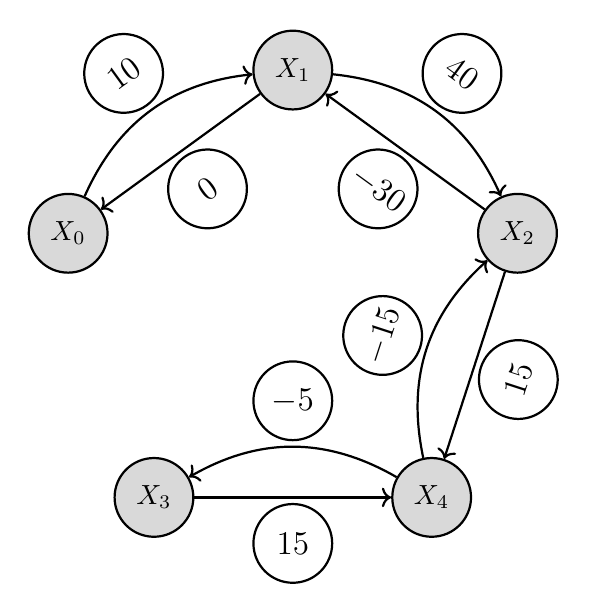
\begin{tikzpicture}[node distance=2cm, every node/.style={circle, draw, minimum size=1cm, inner sep=0pt}, thick]
% Nodes placed in a pentagon shape
\node[fill=gray!30] (X1) at (90:3cm) {$X_1$}; % Top
\node[fill=gray!30] (X0) at (162:3cm) {$X_0$}; % Top-left
\node[fill=gray!30] (X3) at (234:3cm) {$X_3$}; % Bottom-left
\node[fill=gray!30] (X4) at (306:3cm) {$X_4$}; % Bottom-right
\node[fill=gray!30] (X2) at (18:3cm) {$X_2$}; % Top-right
% Edges following the graph structure
\draw[-> , bend left] (X0) to node[sloped,midway,above=0.2em] {\large $10$} (X1) ;
\draw[->] (X1) to node[sloped,midway,below=0.2em] {\large $0$} (X0) ;
\draw[-> , bend left] (X1) to node[sloped,midway,above=0.2em] {\large $40$} (X2) ;
\draw[->] (X2) to node[sloped,midway,below=0.2em] {\large $-30$} (X1) ;
\draw[-> , bend left] (X4) to node[sloped,midway,above=0.2em] {\large $-15$} (X2) ;
\draw[->] (X2) to node[sloped,midway,below=0.2em] {\large $15$} (X4) ;
\draw[-> , bend right] (X4) to node[sloped,midway,above=0.2em] {\large $-5$} (X3) ;
\draw[->] (X3) to node[sloped,midway,below=0.2em] {\large $15$} (X4) ;
\end{tikzpicture}
\end{center}
\end{itemize}
Ο γραφος εχει οσες κορυφες οσες και οι μεταβλητες του προβληματος και δυο μεταβλητες συνδεονται με μια ακμη εαν εμπλεκονται σε καποιον περιορισμο. Επισης για να καταλαβουμε ποιο ειναι το βαρος καθε ακμης ($X_i,X_j$) θα πρεπει να παμε στην ανισοση που συνδεει αυτες τις δυο μεταβλητες. Οι ανισοσεις για καθε ζευγαρι μεταβλητων ειναι οι παρακατω:\\
\newline
$0 \le X_1 - X_0 \le 10$\\
$30 \le X_2 - X_1 \le 40$\\
$5 \le X_4 - X_3 \le 15$\\
$15 \le X_4 - X_2 \le 15$\\
\newline 
Για να βρουμε παραδειγματος χαρη το βαρος της ακμης ($X_0 , X_1$) παιρνουμε τον μεγαλυτερο αριθμο απο τα ακρα της ανισοσης $0 \le X_1 - X_0 \le 10$ , που στην συγκεκριμενη περιπτωση ειναι το $10$ . Αντιθετα για να βρουμε το βαρος της ακμης $(X_1 , X_0)$ περνουμε την μεγαλυτερη τιμη απο τα δυο ακρα της ανισοσης οταν την εχουμε πολλαπλασιασει με το $-1$ , αρα εφοσον το $0 > -10$ το βαρος της ακμης $(X_1 , X_0)$ ειναι το $0$ . Κανουμε την ιδια διαδικασια και για τις υπολοιπες ακμες και προκυπτει ο παραπανω γραφος.\\
\newline
$\bullet$ Ερωτημα $5$:\\
\newline
Εαν εφαρμοσουμε τον αλγοριθμο Floyd-Warhall all pairs-shortest-paths σε ενα απλο χρονικό πρόβλημα, προκύπτει ένα πρόβλημα το οποίο είναι n-consistent(οπου n το πληθος των μεταβλητων). Γνωριζουμε οτι ενα  απλο χρονικο προβλημα ειναι συνεπες εαν στον γραφο αποστασεων δεν υπαρχει αρνητικος κυκλος , δηλαδη κυκλος οπου το συνολικο αθροισμα απο τα βαρη των ακμων του να ειναι αρνητικο. Επειδη ομως ο αλγοριθμος του Floyd εντοπιζει τους αρνητικους κυκλους που προκαλουν αυτην την ασυνεπεια μπορουμε να συμπερανουμε οτι εαν δεν βρει καποιον τετοιο κυκλο τοτε το προβλημα που θα προκυψει μετα την εφαρμογη του αλγοριθμου θα ειναι n-consistent δηλαδη θα ειναι συνεπες σε ολα τα επιπεδα , αφου θα ειμαστε σιγουροι οτι δεν υπαρχουν αρνητικοι κυκλοι.\\
\newpage
$\bullet$ \underline{Σχεδιαστικες Επιλογες}:\\
\newline
\newline
-\underline{Csp.py file}:\\
\newline
Οι τροποποιησεις που εχω κανει στο αρχειο csp.py αφορουν τον variable ordering αλγοριθμο $\frac{dom}{wdeg}$\\
\newline
Συγκεκριμενα:\\
\newline
Εχω προσθεσει σαν πεδιο στην κλαση CSP ενα dictionary με ονομα weight στο οποιο αποθηκευω κλειδια της μορφης $(X_i , X_j)$ οπου $X_i$ και $X_j$ ειναι μεταβλητες του προβληματος που συνδεονται με καποιον περιορισμο και σαν value εχω το βαρος του συγκεκριμενου περιορισμου. Ολα τα βαρη εχουν αρχικοποιηθει στο $1$.\\
\newline
Επισης στον αλγοριθμο forward checking στο σημειο που καταλαβαινουμε οτι το πεδιο της μεταβλητης B εχει αδειασει αυξανω το βαρος του περιορισμου (B , var) κατα 1 . Το ιδιο ισχυει και για τον αλγοριθμο mac οπου στην συναρτηση revise εχω προσθεσει εναν επιπλεον ελεγχο που τσεκαρει εαν το domain της μεταβλητης $X_i$ εχει αδειασει και τοτε αυξανω κατα 1 το βαρος του αντιστοιχου περιορισμου . Επισης στην συναρτηση mac καλω σαν constraint propagation τον AC3 και οχι τον AC3b γιατι αλλιως δεν θα καλεστει ποτε η συναρτηση revise (που ειναι και η συναρτηση στην οποια αυξανονται τα weights στο paper).\\
\newline
Οσον αφορα τον αλγοριθμο $\frac{dom}{wdeg}$ ο στοχος ειναι να επιστρεψουμε την μεταβλητη με την μικροτερη τιμη $\frac{dom}{wdeg}$. Για να γινει αυτο τρεχουμε μια επαναληψη για καθε μεταβλητη του προβληματος και υπολογιζουμε το αθροισμα των weights που περιλαμβανουν την μεταβλητη και τον αντοιστιχο γειτονα της. Στην συνεχεια διαιρουμε (εφοσον ειναι διαφορο του μηδενος αλλιως το θεωρουμε μοναδα) με το αθροισμα των weights των περιορισμων της μορφης $(X_i , X_j)$ οπου $X_i$ ειναι η μεταβλητη που εξεταζουμε και κραταμε παραλληλα και ενα min στο οποιο αποθηκευουμε την μικροτερη τιμη $\frac{dom}{wdeg}$ , επιστρεφωντας στο τελος την μεταβλητη που αντιστοιχει σε αυτην. Εαν δεν βρουμε καποια τετοια μεταβλητη τοτε καλουμε την συναρτηση first unassigned variable η οποια θα επιστεψει μια μεταβλητη με βαση το deafult variable order.\\
\newline
-\underline{Schedule.py file}:\\
\newline
ΣΗΜΑΝΤΙΚΟ: ΓΙΑ ΝΑ ΤΡΕΞΕΤΕ ΕΝΑΝ ΑΛΓΟΡΙΘΜΟ ΘΑ ΠΡΕΠΕΙ ΝΑ ΤΟΝ ΒΓΑΛΕΤΕ ΑΠΟ ΣΧΟΛΙΟ ΜΕΣΑ ΣΤΟ ΠΡΟΓΡΑΜΜΑ\\
\newline
Αποφασισα να μοντελοποιησω το προγραμμα φτιανωντας μια κλαση Exam timetabling η οποια κληρωνομει την CSP. Μεσα σε αυτην την κλαση οριζω τις μεταβλητες του προβληματος , το domain καθε μεταβλητης , τους γειτονες της , την συναρτηση Exam constraints μεσα στην οποια ελεγχω εαν ικανοποιουνται ολοι οι περιορισμοι μεταξυ δυο μεταβλητων A και B . Τελος καλω τον constructor του CSP στον οποιο περναω σαν παραμετρους τις μεταβλητες , τα domains , τα neighbors και την constraint function.\\
\newline
Οι μεταβλητες του προβληματος ειναι τα 38 ονοματα των μαθηματων(Τα εργαστηρια δεν τα μετραω ως ξεχωριστο μαθημα)\\
\newline
Το domain καθε μεταβλητης αποφασισα να ειναι ολοι οι δυνατοι συνδιασμοι μερας και ωρας σαν string της μορφης "day κατω παυλα time" . Για να παρω την μερα και την ωρα κανω split το string.\\
\newline
Καθε μεταβλητη εχει σαν γειτονα ολες τις υπολοιπες αφου εχουμε μονο μια αιθουσα και σε καθε ωρα μπορουμε να εξεταζουμε μονο ενα μαθημα. \\
\newline
Επισης εχω ενα dictionary με ονομα other data στο οποιο κανω μια αντιστοιχιση μεταξυ μεταβλητης και μιας λιστας που περιεχει το ονομα του καθηγητη που διδασκει το μαθημα, το εξαμηνο του μαθηματος , εαν ειναι δυσκολο ή οχι και εαν εχει Lab.
\\
\newline
Οσον αφορα την συναρτηση Exam constraints πρεπει να δωσουμε ιδιαιτερη προσοχη στα μαθηματα που εχουν Lab καθως πρεπει να εξεταζονται αμεσως μετα την θεωρια. Ο ελεγχος αυτος γινεται με το να τσεκαρουμε εαν μετα την εξεταση της θεωριας δεν εξεταζεται το μαθημα B που εχουμε σαν δευτερη μεταβλητη στην συναρτηση, ή εαν το μαθημα της θεωριας εξεταζεται στις 3-6 τοτε σημαινει οτι δεν υπαρχει διαθεσιμο slot για την εξεταση του Lab αρα θα πρεπει να επιστρεψουμε False. Εαν και τα δυο μαθηματα εχουν εργαστηριο και εξεταζονται την ιδια μερα τοτε ειναι αδυνατο να εξεταστει και η θεωρια και το Lab του αντιστοιχου μαθηματος καθως εχουμε μονο $3$ διαθεσιμα slots για καθε μερα. Φυσικα μαθηματα ιδιου εξαμηνου , ιδιου καθηγητη πρεπει να εξεταζονται σε διαφορετικες μερες , οπως και τα hard μαθηματα πρεπει να απεχουν τουλαχιστον δυο μερες.\\
\newline
Τελος εχω φτιαξει μια συναρτηση Print Result η οποια τυπωνει το τελικο προγραμμα της εξεταστικης ξεκινωντας απο την μερα $1$.\\
\newline
-\underline{Floyd.py file}:\\
\newline
Δεν εχω να προσθεσω κατι , εχω παραθεσει αναλυτικα σχολια μεσα στον κωδικα.
\end{document}



